This chapter discusses the performance level of a single ipvs load balancer.
First the author investigated general characteristics of a single load balancer using physical servers in on-premise data center and compared performance level with existing iptables DNAT and nginx as a load balancer within a 1Gbps network environment.
Then the author also carried out the performance measurement in GCP and AWS to show that the containerized ipvs load balancer is runnable and has the same characteristics in the cloud environment.
Furthermore, experiment was extended into the 10Gbps network environment to investigate the performance limitations of the proposed load balancer and to explore methods to improve them.
The following sections explain these in further detail.

\section{On-premise experiment with 1Gbps Load balancer}
\subsection{Benchmark method}

A set of throughput measurement was carried out using an HTTP benchmark program, wrk\cite{Glozer2016}.
Figure~\ref{fig:benchmark-setup}(\subref{fig:benchmark-schem}) illustrates a schematic diagram of the experimental setup.
Multiple {\em pods} are deployed on multiple nodes in the Kubernetes cluster. 
In each {\em pod}, an nginx web server pod that returns the IP address of the {\em pod} are running.
The author set up the ipvs, iptables DNAT, and nginx load balancers on one of the nodes.
All the nodes and the benchmark client are connected to a 1Gbps network switch as in Figure~\ref{fig:benchmark-setup}(\subref{fig:bench_1g}).

The throughput, Request/sec, is measured cluster as follows:
The HTTP GET requests are sent out by the wrk on the client machine toward the nodes,
using destination IP addresses and port numbers that are chosen based on the type of the load balancer on which the measurement is performed.
The load balancer on the node then distributes the requests to the {\em pods}.
Each {\em pod} returns HTTP responses to the load balancer, after which the load balancer returns them to the client.
Based on the number of responses received by wrk on the client, 
load balancer performance, in terms of Request/sec can be obtained. 

\begin{figure}
\begin{subfigure}[t]{\columnwidth}
  \centering
  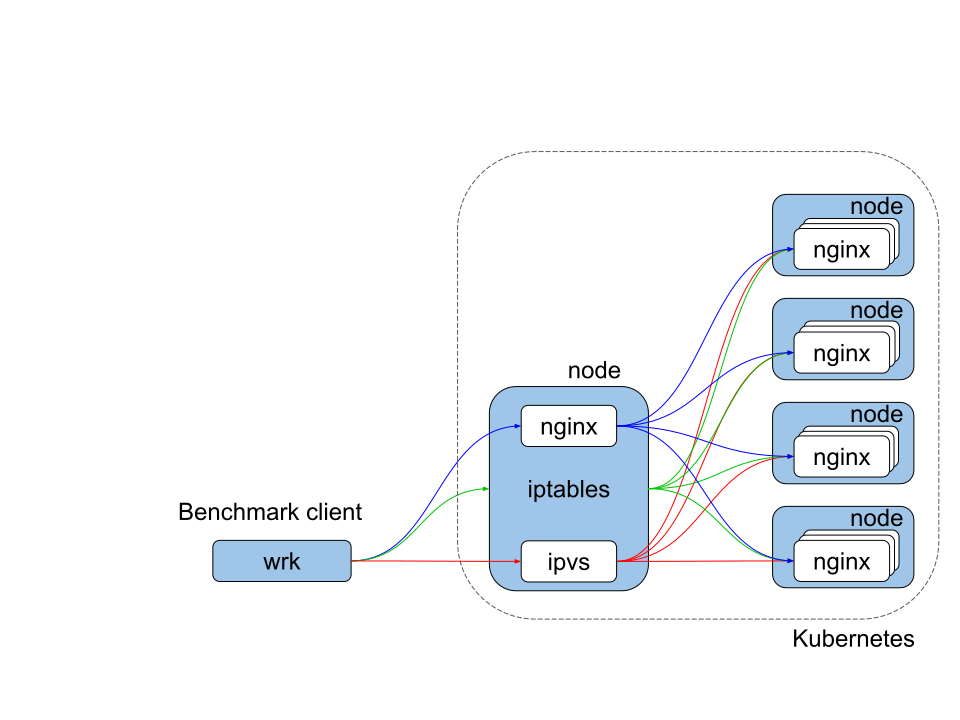
\includegraphics[width=0.8\columnwidth]{Figs/benchmark-schem}
  \vspace{1cm}
  \caption{Logical configuration.}
  \label{fig:benchmark-schem}
\end{subfigure}
  \vspace{1cm}

\begin{subfigure}[t]{\columnwidth}
  \centering
  \includegraphics[width=0.8\columnwidth]{Figs/bench_1g}
  \vspace{1cm}
  \caption{Physical configuration.}
  \label{fig:bench_1g}
\end{subfigure}
  \caption{Benchmark setup. }
  \label{fig:benchmark-setup}
\end{figure}

Table~\ref{tab:bench_example} shows an example of the command-line for wrk and the corresponding output.
The command-line in Table~\ref{tab:bench_example} will generate 40 wrk program threads and allow those threads to send out a total of 800 concurrent HTTP requests over the period of 30 seconds.
The output example shows the information including per thread statistics, error counts, Request/sec and Transfer/sec.

\begin{table}[h]
  \centering
  \begin{tabular}{l}
    \hline
    \begin{minipage}{13cm}
      \begin{verbatim}

[Command line] 
 wrk -c800 -t40 -d30s http://172.16.72.2:8888/ 
-c: concurrency, -t: # of thread, -d: duration 

[Output example] 
 Running 30s test @ http://10.254.0.10:81/ 
  40 threads and 800 connections 
  Thread Stats   Avg      Stdev     Max   +/- Stdev 
    Latency    15.82ms   41.45ms   1.90s    91.90\% 
    Req/Sec     4.14k   342.26     6.45k    69.24\% 
  4958000 requests in 30.10s, 1.14GB read 
  Socket errors: connect 0, read 0, write 0, timeout 1 
Requests/sec: 164717.63 
Transfer/sec:     38.86MB 
      \end{verbatim}
    \end{minipage}
   \\ \hline
  \end{tabular}
  \caption{}
  \label{tab:bench_example}
\end{table}

Table~\ref{tab:hw_sw_spec} shows hardware and software configuration used in the experiments.
%Physical servers with the same specification are used for nodes(nginx, load balancer) and benchmark client.
All of the nginx web server pods are configured to return the IP address of the {\em pod}, in order to make them return a small HTTP content. This makes a relatively severe condition for load balancers. 
The size of the character string making up an IP address is limited to 15 bytes.
If the author had chosen the HTTP response size so that most of the IP packet resulted in maximum transmission unit(MTU), the performance would have been dominantly limited by the Ethernet bandwidth.
% However, since small HTTP responses are used, the auhtor could purely measure the load balancer performance.

\begin{table}[]
  \centering
  \begin{tabular}{ll}
    \hline 
    \multicolumn{2}{l}{[Hardware Specification]}   \\
    & CPU: Xeon E5-2450 2.10GHz (with 8 core, Hyper Threading) \\
    & Memory: 32GB \\
    & NIC: Broadcom BCM5720 Giga bit \\
    & (Node x 6, LB x 1, Client x 1) \\
    & \\
    \multicolumn{2}{l}{[Node Software]}  \\
    & OS: Debian 8.7, linux-3.16.0-4-amd64 \\
    & Kubernetes v1.10.6 \\
    & flannel v0.7.0 \\
    & etcd version: 3.0.15 \\
    & \\
    \multicolumn{2}{l}{[Container Software]}   \\
    & Keepalived: v1.3.2 (12/03,2016) \\
    & nginx : 1.11.1(load balancer), 1.13.0(web server) \\
    \hline
  \end{tabular}
  \caption{}
  \label{tab:hw_sw_spec}
\end{table}

For this experiment a total of eight servers are used; six servers for nodes, one for the load balancer and one for the benchmark client, with all having the same hardware specifications.
The software versions used for Kubernetes, web server and load balancer {\em pods} are also summarized in the Table~\ref{tab:hw_sw_spec}.
The hardware we used had eight physical CPU cores and a 1Gbps NIC with 4 rx-queues.

\subsection{Result 1: Effect of multicore proccessing}

\begin{figure}
  \centering
  \includegraphics[width=0.8\columnwidth]{Figs/ipvs_mcore_proccessing}
  \caption{Effect of multicore proccessing on ipvs throughput.}
  \label{fig:ipvs_mcore_proccessing}
\end{figure}

Figure~\ref{fig:ipvs_mcore_proccessing} shows the effect of multicore proccessing.
The following three RSS and RPS settings were compared: 
\begin{center}
  \centering
  \begin{minipage}{0.8\columnwidth}
\begin{verbatim}
(RSS, RPS) = (off, off)
           = (on , off)
           = (off, on )
\end{verbatim}
  \end{minipage}
\end{center}
The host-gw mode of flannel backends is used as the overlay network.

The case with \enquote{(RSS, RPS) = (off, off)} means that all the incomming packets are processed by single core. 
The \enquote{(RSS, RPS) = (on, off)} means that the packet proccessing is done on 4 of the CPU cores since the NIC used in the experiment has only four rx-queues. 
The \enquote{(RSS, RPS) = (off, on)} means that all of the CPU cores are utilized for the packet proccessing.

We can see a general trend in which the throughput linearly increases as the number of nginx {\em pod}s increases and then it eventually saturates.
The saturated throughput levels indicate the maximum performance level of the ipvs load balancer.
The maximum performance levels depend on the (RSS, RPS) settings.
From the results in this figure, it can be seen that if we turn off multicore packet processing,
{\it i.e.}, when \enquote{(RSS, RPS) = (off, off)}, performance degrades significantly.
In this case, the performance bottleneck is primarily due to packet processing in a single core.

If we compare the results for the cases when \enquote{(RSS, RPS) = (on, off)} and \enquote{(RSS, RPS) = (off, on)},
the latter is better than the former.
It is clear that the case that utilizes all of the CPU cores better performs than the case with only four CPU cores utilized. 

\begin{figure}[h]
  \centering
  \includegraphics[width=0.8\columnwidth]{Figs/tp_limit_1gbps}
  \caption{Performance limitation due to 1Gbps bandwidth}
  \label{fig:performance_limitation}
\end{figure}

At first, it was not clear what caused the performance limit for the case when \enquote{(RSS, RPS) = (off, on)},
however it now turned out to be due to 1Gbps bandwidth limitation.
A packet level analysis using tcpdump\cite{jacobson1989tcpdump} revealed that 665.36 byte of extra HTTP headers, 
TCP/IP headers and ethernet frame headers are needed for each request in the case of the wrk benchmack program(Appendix~\ref{}). 
This results in the upper limitation of 184,267 [req/sec], when the date size of HTTP response body is 13 byte, or typical data size in our experiment. 
Figure~\ref{fig:performance_limitation} shows theoretical upper limitation of the performance level for 1Gbps ethernet together with actual benchmark results and they agree well.
Therefore it can be said that when \enquote{RPS = on}, ipvs performance is limited by 1Gbps bandwidth.
The author regarded that \enquote{(RSS, RPS) = (off, on)} is the best setting in our experimental conditions, and used this setting throughout this thesis unless explicitly stated otherwise.

\FloatBarrier

\subsection{Result 2: Effect of overlay network}

\begin{figure}[h]
  \centering
  \includegraphics[width=0.8\columnwidth]{Figs/ipvs_flannel_mode}
  \caption{Effect of flannel backend modes on ipvs throughput.}
  \label{fig:ipvs_flannel_mode}
\end{figure}

Figure~\ref{fig:ipvs_flannel_mode} shows the effect of flannel backend modes on ipvs throughput.
As for the overlay network, the author measured the performance levels for three flannel backend modes, host-gw, vxlan and udp.
Except for the udp case, we can see the trend in which the throughput linearly increases 
as the number of nginx {\em pod} increases and then it eventually saturates.
The saturated throughput levels indicate the maximum performance levels of the ipvs load balancer.
If we compare the performance levels among the flannel backend modes types, 
the host-gw mode where no encapsulation is conducted shows the highest performance level,
followed by the vxlan mode where the Linux kernel encapsulate the Ethernet frame.
The udp mode where flanneld itself encapsulate the IP packet shows significantly lower performances levels.
The author considers the host-gw mode is the best, the vxlan tunnel the second best and the udp tunnel mode unusable.

\FloatBarrier

\subsection{Result 3: Comparison of different load balancer}

\begin{figure}[htb]
  \centering
  \includegraphics[width=0.8\columnwidth]{Figs/ipvs-iptables-nginx}
  \caption{Throughput comparison between ipvs, iptables DNAT and nginx.}
  \label{fig:ipvs-iptables-nginx}
\end{figure}

\begin{figure}[htb]
  \centering
  \includegraphics[width=0.8\columnwidth]{Figs/latency_cdf_rps_40pods}
  \caption{Latency cumulative distribution function.}
  \label{fig:latency_cdf_rps_40pods}
\end{figure}

Figure~\ref{fig:ipvs-iptables-nginx} compares the performance measurement results among the ipvs, iptables DNAT, and Nginx load balancers.
The proposed ipvs load balancer exhibits almost equivalent performance as the iptables DNAT based load balancer. 
The Nginx based load balancer shows no performance improvement even though the number of the Nginx web server {\em pods} is increased.
It is understandable because the performance of the single nginx as a load balancer is expected to be similar to the performance as a web server.

Figure~\ref{fig:latency_cdf_rps_40pods} compares Cumulative Distribution Function(CDF) of the load balancer latency at the two constant loads, 160K[req/sec] and 180K[req/sec].
We can see that the latencies are a little bit smaller for ipvs.
For example, the median value at 160K[req/sec] load for ipvs and iptables DNAT are, 1.1 msec and 1.2 msec, respectively.
This may not be considered a siginificant difference, however we can at least say that our proposed load balancer are as good as iptables DNAT.
So, to conclude this section, the containerized ipvs load balancer showed equivalent performance leves with the iptables DNAT loadbalancing functions that is used in Kubernetes cluster.

\FloatBarrier

\section{Cloud experiment}

\begin{figure}[t]
  \centering
  \includegraphics[width=0.8\columnwidth]{Figs/gcp_all_tp}
  \caption{GCP}
  \label{fig:gcp_all_ieice}
\end{figure}

\begin{figure}[t]
  \centering
  \includegraphics[width=0.8\columnwidth]{Figs/aws_c4_tp}
  \caption{AWS with Node x 6, Client x 1, Load balancer x 1. Custom instance. }
  \label{fig:aws_c4_ieice}
\end{figure}

Fig.~\ref{fig:ipvs_performance}~(\subref{fig:gcp_all_ieice}) and Fig.~\ref{fig:ipvs_performance}~(\subref{fig:aws_c4_ieice}) show the load balancer performance levels that are measured in GCP and AWS, respectively.
These are aimed to show that our proposed load balancer can be run in cloud environments and also functions properly.

Both results show similar characteristics as the experiment in an on-premise data center in Fig.~\ref{fig:ipvs_performance}~(\subref{fig:ipvs-iptables-nginx}), where throughput increased linearly to a certain saturation level that is determined by either network speed or machine specifications.
Since in the cases of cloud environments we can easily change the machine specifications, especially CPU counts, we measured throughput with several conditions of them.
From the first look of the results, since changing CPU counts changed the load balancer's throughput saturation levels, we thought VM's computation power limited the performance levels.
However, since there are cases in the cloud environment, where changing the VM types or CPU counts also changes the network bandwidth limit, a detailed analysis is further required in the future to clarify which factor limits the throughput in the cases of these cloud environments.
Still, we can say that the proposed ipvs load balancers can be run in GCP and AWS, and function properly until they reach the infrastructure limitations.

\FloatBarrier

\section{Summary}



